\chapter{Graphics}

\section{Meshes}\label{sec:Mesh-graphics}

In case you used the internal mesher \texttt{xmeshfem3D} to create
and partition your mesh, you can output mesh files in ABAQUS (.INP)
and DX (.dx) format to visualize them. For this, you must set either
the flag \texttt{CREATE\_DX\_FILES} or \texttt{CREATE\_ABAQUS\_FILES}
to \texttt{.true.} in the mesher's parameter file \texttt{Mesh\_Par\_file}
prior to running the mesher (see Chapter~\ref{cha:Running-the-Mesher-Meshfem3D}
for details). You can then use AVS \urlwithparentheses{www.avs.com}
or OpenDX \urlwithparentheses{www.opendx.org} to visualize the mesh
and MPI partition (slices).

\begin{figure}[htbp]
\noindent \begin{centering}
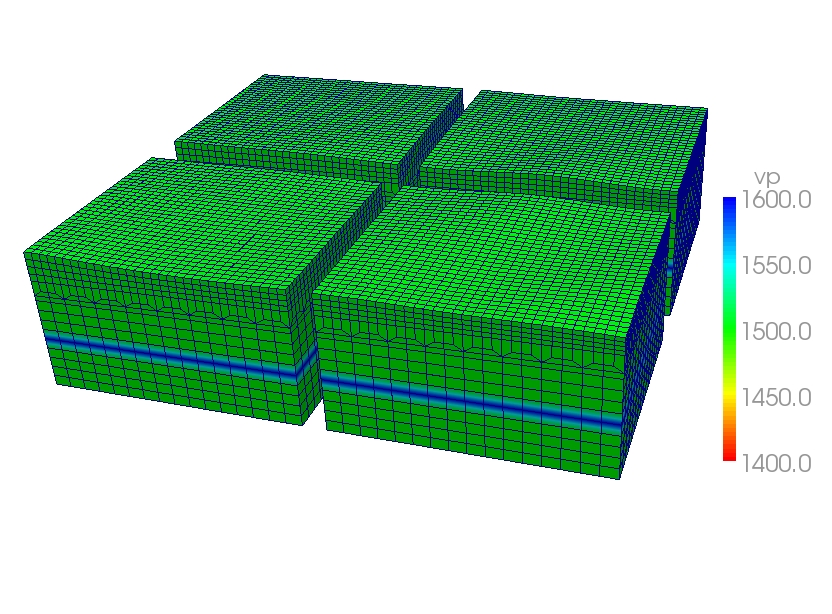
\includegraphics[width=0.49\textwidth]{figures/vtk_mesh_vp.jpg}
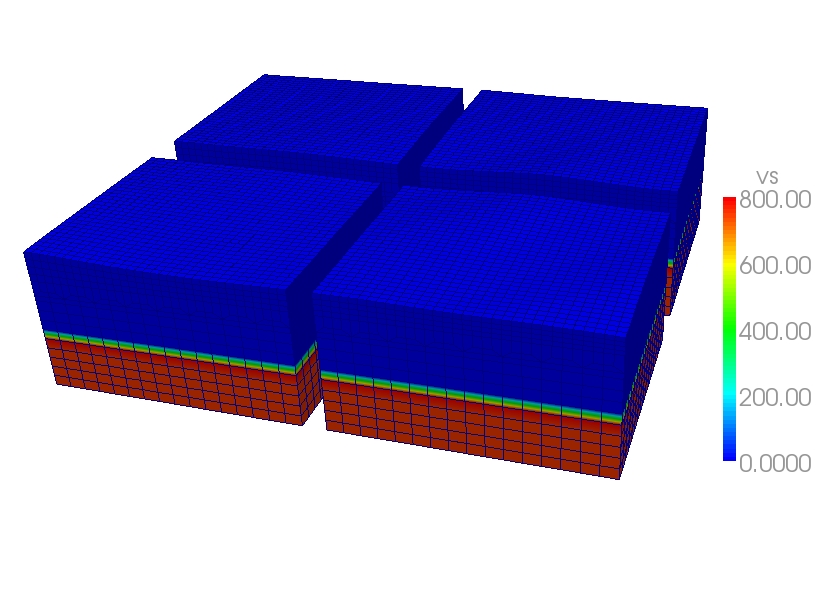
\includegraphics[width=0.49\textwidth]{figures/vtk_mesh_vs.jpg}
\par\end{centering}

\caption{Visualization using Paraview of VTK files created by \texttt{xgenerate\_databases}
showing P- and S-wave velocities assigned to the mesh points. The
mesh was created by \texttt{xmeshfem3D} for 4 processors.}


\label{fig:vtk.mesh}
\end{figure}


You have also the option to visualize the distributed databases produced
by \texttt{xgenerate\_databases} using Paraview \urlwithparentheses{www.paraview.org}.
For this, you must set the flag \texttt{SAVE\_MESH\_FILES} to \texttt{.true.}
in the main parameter file \texttt{Par\_file} (see Chapter~\ref{cha:Main-Parameter}
for details). This will create VTK files for each single partition.
You can then use Paraview \urlwithparentheses{www.paraview.org}
to visualized these partitions.


\section{Movies}\label{sec:Movies}

To make a surface or volume movie of the simulation, set parameters
\texttt{MOVIE\_SURFACE}, \texttt{MOVIE\_VOLUME}, \texttt{MOVIE\_TYPE},
and \texttt{NTSTEP\_BETWEEN\_FRAMES} in the \texttt{Par\_file}. Turning
on the movie flags, in particular \texttt{MOVIE\_VOLUME}, produces
large output files. \texttt{MOVIE\_VOLUME} files are saved in the
\texttt{LOCAL\_PATH} directory, whereas \texttt{MOVIE\_SURFACE} output
files are saved in the \texttt{OUTPUT\_FILES} directory. We save the
displacement field if the parameter \texttt{SAVE\_DISPLACEMENT} is
set, otherwise the velocity field is saved. The look of a movie is
determined by the half-duration of the source. The half-duration should
be large enough so that the movie does not contain frequencies that
are not resolved by the mesh, i.e., it should not contain numerical
noise. This can be accomplished by selecting a CMT \texttt{HALF\_DURATION}
> 1.1 $\times$ smallest period (see figure \ref{fig:CMTSOLUTION-file}).
When \texttt{MOVIE\_SURFACE} = .\texttt{true.}, the half duration
of each source in the \texttt{CMTSOLUTION} file is replaced by
\begin{quote}
\[
\sqrt{(}\mathrm{\mathtt{HALF\_DURATIO}\mathtt{N}^{2}}+\mathrm{\mathtt{HDUR\_MOVI}\mathtt{E}^{2}})
\]
 \textbf{NOTE:} If \texttt{HDUR\_MOVIE} is set to 0.0, the code will
select the appropriate value of 1.1 $\times$ smallest period. As
usual, for a point source one can set \texttt{half duration} in the
\texttt{CMTSOLUTION} file to be 0.0 and \texttt{HDUR\_MOVIE} = 0.0
in the \texttt{Par\_file} to get the highest frequencies resolved
by the simulation, but for a finite source one would keep all the
\texttt{half durations} as prescribed by the finite source model and
set \texttt{HDUR\_MOVIE} = 0.0.
\end{quote}

\subsection{Movie Surface}

When running \texttt{xspecfem3D} with the \texttt{MOVIE\_SURFACE}
flag turned on, the code outputs \texttt{moviedata??????} files in
the \texttt{OUTPUT\_FILES} directory. There are several flags in the
main parameter file \texttt{Par\_file} that control the output of
these movie data files (see section \ref{cha:Main-Parameter} for
details):
\texttt{\small NTSTEP\_BETWEEN\_FRAMES} to set the
timesteps between frames,
\texttt{\small SAVE\_DISPLACEMENT}
to save displacement instead of velocity,
\texttt{\small USE\_HIGHRES\_FOR\_MOVIES}
to save values at all GLL point instead of element edges. In order
to output additionally shakemaps, you would set the parameter
\texttt{\small CREATE\_SHAKEMAP}
to \texttt{\small .true.}.

The files are in a fairly complicated binary format, but there is
a program provided to convert the output into more user friendly formats:
\begin{description}
\item [{\texttt{xcreate\_movie\_shakemap\_AVS\_DX\_GMT}}]
From \texttt{create\_movie\_shakemap\_AVS\_DX\_GMT.f90},
it outputs data in ASCII, OpenDX, or AVS format (also readable in
ParaView). Before compiling the code, make sure you have the file
\texttt{surface\_from\_mesher.h} in the \texttt{OUTPUT\_FILES/} directory.
This file will be created by the solver run. Then type

{\footnotesize
\begin{verbatim}
make xcreate_movie_shakemap_AVS_DX_GMT
\end{verbatim}
}
and run the executable \texttt{xcreate\_movie\_shakemap\_AVS\_DX\_GMT}
in the main directory. It will create visualization files
in your format of choice. The code will prompt the user for input
parameters.


\begin{figure}[htbp]
\noindent \begin{centering}
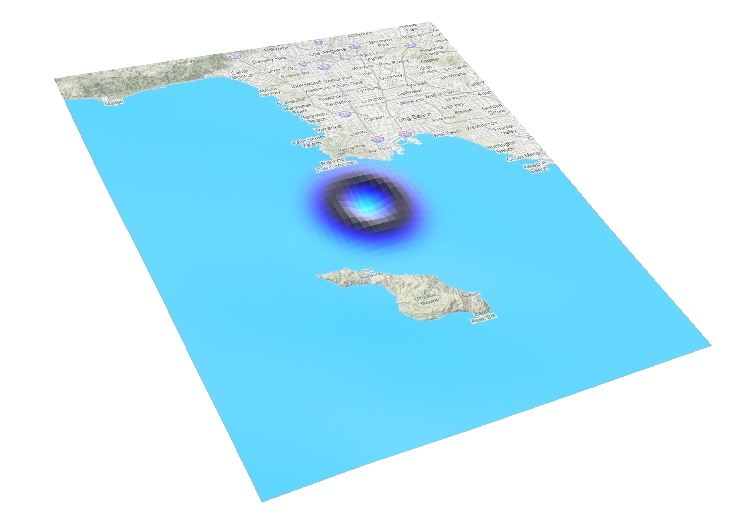
\includegraphics[width=0.32\textwidth]{figures/movie_surf_1.jpg}
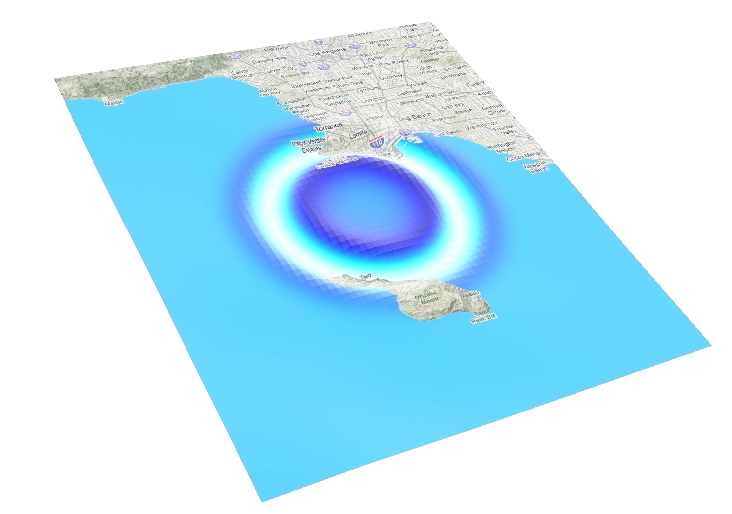
\includegraphics[width=0.32\textwidth]{figures/movie_surf_2.jpg}
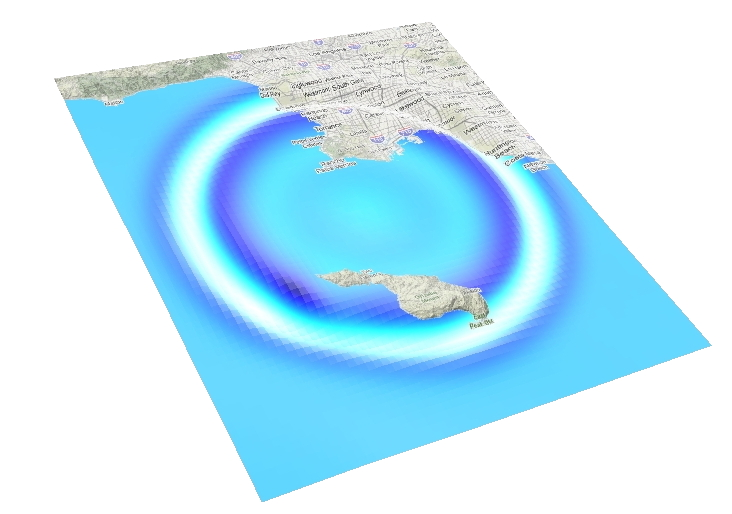
\includegraphics[width=0.32\textwidth]{figures/movie_surf_3.jpg}
\par\end{centering}

\caption{Visualization using AVS files created by \texttt{xcreate\_movie\_shakemap\_AVS\_DX\_GMT}
showing movie snapshots of vertical velocity components at different
times.}


\label{fig:movie.surf}
\end{figure}


\end{description}
The \texttt{SPECFEM3D Cartesian} code is running in near real-time
to produce animations of southern California earthquakes via the web;
see Southern California ShakeMovie\textregistered{}\urlwithparentheses{www.shakemovie.caltech.edu}.


\subsection{Movie Volume}\label{sub:Movie-Volume}

When running xspecfem3D with the
\texttt{\small MOVIE\_VOLUME}
flag turned on, the code outputs several files in \texttt{\small LOCAL\_PATH}
specified in the main \texttt{\small Par\_file},
e.g. in directory \texttt{\small OUTPUT\_FILES/DATABASES\_MPI}.
The output is saved by each processor at the time interval specified
by
\texttt{\small NTSTEP\_BETWEEN\_FRAMES}.
For all domains,
the velocity field is output to files:
{\small
\begin{verbatim}
proc??????_velocity_X_it??????.bin
proc??????_velocity_Y_it??????.bin
proc??????_velocity_Z_it??????.bin
\end{verbatim}
}
For elastic domains, the divergence and curl taken from the velocity field,
i.e. $\nabla\cdot{\bf {v}}$ and $\nabla\times{\bf {v}}$, get stored
as well:
{\small
\begin{verbatim}
proc??????_div_it??????.bin
proc??????_curl_X_t??????.bin
proc??????_curl_Y_it??????.bin
proc??????_curl_Z_it??????.bin
\end{verbatim}
}
The files denoted \texttt{\small proc??????\_div\_glob\_it??????.bin} and
\texttt{\small proc??????\_curl\_glob\_it??????.bin}
are stored on the global points only, all the other arrays are stored
on all GLL points. Note that the components X/Y/Z can change to E/N/Z
according to the
\texttt{\small SUPPRESS\_UTM\_PROJECTION}
flag (see also Appendix~\ref{cha:Coordinates} and \ref{cha:channel-codes}).

\begin{figure}[htbp]
\noindent \begin{centering}
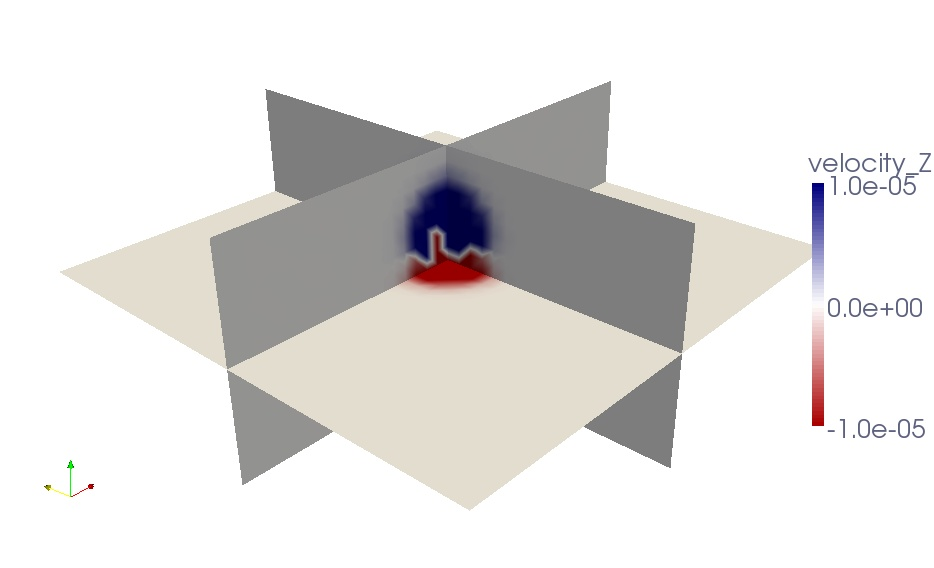
\includegraphics[width=0.32\textwidth]{figures/movie_volume_1.jpg}
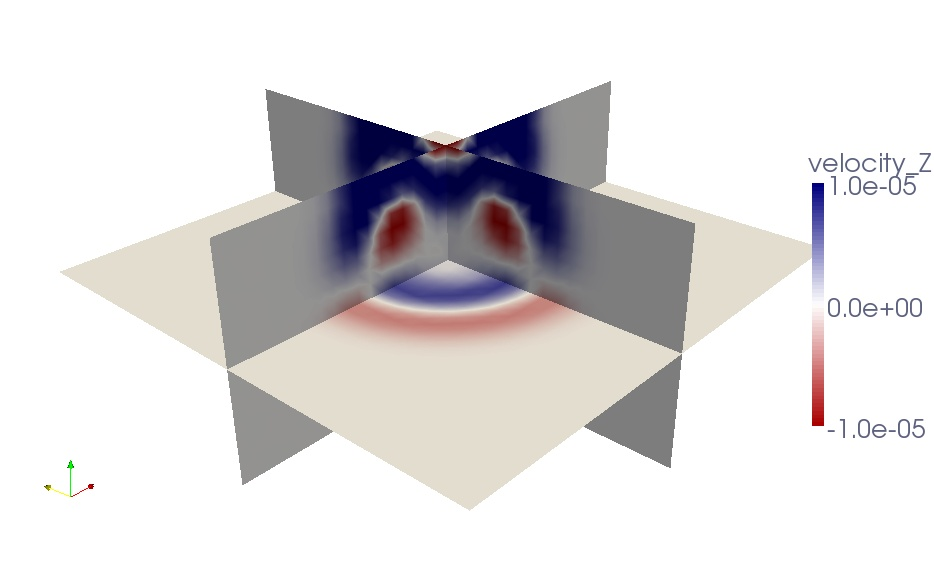
\includegraphics[width=0.32\textwidth]{figures/movie_volume_2.jpg}
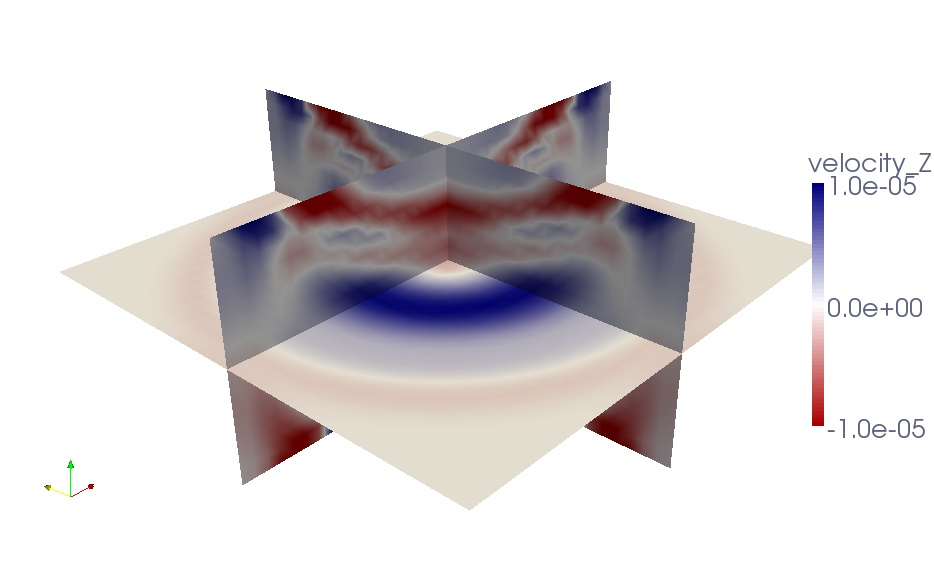
\includegraphics[width=0.32\textwidth]{figures/movie_volume_3.jpg}
\par\end{centering}

\caption{Paraview visualization using movie volume files (converted by \texttt{xcombine\_vol\_data}
and \texttt{mesh2vtu.pl}) and showing snapshots of vertical velocity
components at different times.}


\label{fig:movie.volume}
\end{figure}


To visualize these files, we use an auxilliary program \texttt{combine\_vol\_data.f90}
to combine the data from all slices into one mesh file. To compile
it in the root directory, type:

{\footnotesize
\begin{verbatim}
make xcombine_vol_data
\end{verbatim}
}
which will create the executable \texttt{bin/xcombine\_vol\_data}.
To output the usage of this executable, type
{\footnotesize
\begin{verbatim}
./bin/xcombine_vol_data
\end{verbatim}
}
without arguments.

\medskip

\texttt{xcombine\_vol\_data} will combine the data on the different processors (located in \texttt{OUTPUT\_FILES/DATABASES\_MPI}), for a given quantity and a given iteration, to one file. For example, if you want to combine \texttt{velocity\_Z}, for the iteration 400 on 4 processors, i.e. if you want to combine these files :
{\small
\begin{verbatim}
proc000000_velocity_Z_it000400.bin
proc000001_velocity_Z_it000400.bin
proc000002_velocity_Z_it000400.bin
proc000003_velocity_Z_it000400.bin
\end{verbatim}
}

You have to go in the directory of the concerned example (where are the directories \texttt{DATA}, \texttt{OUTPUT\_FILES}, etc.).
Then, you can launch \texttt{xcombine\_vol\_data}, specifying the path where it is located. As an example, if the \texttt{DATA} and \texttt{OUTPUT\_FILES} directories of the concerned example are in the root specfem3d directory, \texttt{xcombine\_vol\_data} is in \texttt{./bin}, and you have to type:

{\footnotesize
\begin{verbatim}
./bin/xcombine_vol_data 0 3 velocity_Z_it000400 ./OUTPUT_FILES/DATABASES_MPI ./OUTPUT_FILES 0
\end{verbatim}
}
Here, $0$ is the number of the first processor, $3$ the number of the last one, \texttt{velocity\_Z\_it000400} the name of the files we want to combine without the prefix \texttt{proc000000*\_}, \texttt{./OUTPUT\_FILES/DATABASES\_MPI} the directory where the files are located, \texttt{./OUTPUT\_FILES} the directory where the combined file will be stored, and $0$ is the parameter to create a low-resolution mesh file ($1$ for a high-resolution).

\medskip

At the beginning of the source file \texttt{combine\_vol\_data.f90} (located in \texttt{src/auxiliaries/}), there is a logical constant parameter \texttt{USE\_VTK\_OUTPUT} whose default value is \texttt{.true.}, that which will provide the output combined file directly in the VTK format and you can use Paraview to visualize it.

\medskip

If the value of this parameter is \texttt{.false.}, the output mesh file will have the name \texttt{velocity\_Z\_it000400.mesh}. Then we next have to convert the
\texttt{.mesh} file into the VTU (Unstructured grid file) format which can be viewed in ParaView.

\noindent
For this task, you can use and modify the
script \texttt{mesh2vtu.pl} located in directory \texttt{\small utils/Visualization/Paraview/}, for example:

{\footnotesize
\begin{verbatim}
mesh2vtu.pl -i velocity_Z_it000400.mesh -o velocity_Z_it000400.vtu
\end{verbatim}
}

Notice that this Perl script uses a program \texttt{mesh2vtu} in the \texttt{utils/Visualization/Paraview/mesh2vtu} directory, which further
uses the VTK \urlwithparentheses{http://www.vtk.org/} run-time library for its execution. Therefore, make sure you have them properly set
in the script according to your system.

\bigskip

Then, to do a movie with several iterations, you have to repeat this process for each iteration you want to put in your movie.

\section{Finite-Frequency Kernels}\label{sec:Finite-Frequency-Kernels}

The finite-frequency kernels computed as explained in Section \ref{sec:Adjoint-simulation-finite}
are saved in the \texttt{LOCAL\_PATH} at the end of the simulation.
Therefore, we first need to collect these files on the front end,
combine them into one mesh file, and visualize them with some auxilliary
programs.
\begin{enumerate}
\item \textbf{Create slice files}


We will only discuss the case of one source-receiver pair, i.e., the
so-called banana-doughnut kernels. Although it is possible to collect
the kernel files from all slices on the front end, it usually takes
up too much storage space (at least tens of gigabytes). Since the
sensitivity kernels are the strongest along the source-receiver great
circle path, it is sufficient to collect only the slices that are
along or close to the great circle path.


A Perl script \texttt{slice\_number.pl} located in directory \texttt{utils/Visualization/Paraview/}
can help to figure out the slice numbers that lie along the great
circle path. It applies to meshes created with the internal mesher
\texttt{xmeshfem3D}.
\begin{enumerate}
\item On machines where you have access to the script, copy the \texttt{Mesh\_Par\_file},
and \texttt{output\_solver} files, and run:

{\small
\begin{verbatim}
slice_number.pl Mesh_Par_file output_solver.txt slice_file
\end{verbatim}
}
which will generate a \texttt{slices\_file}.

\item For cases with multiple sources and multiple receivers, you need to
provide a slice file before proceeding to the next step.
\end{enumerate}
\item \textbf{Collect the kernel files}


After obtaining the slice files, you can collect the corresponding
kernel files from the given slices.
\begin{enumerate}
\item You can use or modify the script \texttt{utils/copy\_basin\_database.pl}
to accomplish this:

{\small
\begin{verbatim}
utils/copy_database.pl slice_file lsf_machine_file filename [jobid]
\end{verbatim}
}
where \texttt{\small lsf\_machine\_file}{\small{} is the machine file
generated by the LSF scheduler, }\texttt{\small filename}{\small{}
is the kernel name (e.g., }\texttt{\small rho\_kernel}{\small , }\texttt{\small alpha\_kernel}{\small{}
and }\texttt{\small beta\_kernel}{\small ), and the optional }\texttt{\small jobid}{\small{}
is the name of the subdirectory under }\texttt{\small LOCAL\_PATH}{\small{}
where all the kernel files are stored.}{\small \par}

\item After executing this script, all the necessary mesh topology files
as well as the kernel array files are collected to the local directory
of the front end.
\end{enumerate}
\item \textbf{Combine kernel files into one mesh file}


We use an auxilliary program \texttt{combine\_vol\_data.f90} to combine
the kernel files from all slices into one mesh file.
\begin{enumerate}
\item Compile it in the root directory:
{\footnotesize
\begin{verbatim}
make xcombine_vol_data
./bin/xcombine_vol_data slice_list filename input_dir output_dir high/low-resolution
\end{verbatim}
}
where \texttt{input\_dir} is the directory where all the individual
kernel files are stored, and \texttt{output\_dir} is where the mesh
file will be written.

\item Use 1 for a high-resolution mesh, outputting all the GLL points to
the mesh file, or use 0 for low resolution, outputting only the corner
points of the elements to the mesh file.
\item The output mesh file will have the name \texttt{filename\_rho(alpha,beta).mesh}
\end{enumerate}

\item \textbf{Convert mesh files into .vtu files}

\begin{enumerate}
\item We next convert the \texttt{.mesh} file into the VTU (Unstructured
grid file) format which can be viewed in ParaView. For this task,
you can use and modify the script \texttt{mesh2vtu.pl} located in
directory \texttt{utils/Visualization/Paraview/}, for example:

{\footnotesize
\begin{verbatim}
mesh2vtu.pl -i file.mesh -o file.vtu
\end{verbatim}
}

\item Notice that this Perl script uses a program \texttt{mesh2vtu} in the
\texttt{\small utils/Visualization/Paraview/mesh2vtu} directory, which further
uses the VTK \urlwithparentheses{http://www.vtk.org/} run-time library
for its execution. Therefore, make sure you have them properly set
in the script according to your system.
\end{enumerate}

\item \textbf{Copy over the source and receiver .vtk file}


In the case of a single source and a single receiver, the simulation
also generates the file \texttt{sr.vtk} located in the \texttt{OUTPUT\_FILES/}
directory to describe the source and receiver locations, which can
also be viewed in Paraview in the next step.

\item \textbf{View the mesh in ParaView}


Finally, we can view the mesh in ParaView \urlwithparentheses{www.paraview.org}.
\begin{enumerate}
\item Open ParaView.
\item From the top menu, \textsf{File} $\rightarrow$\textsf{Open data},
select \texttt{file.vtu}, and click the \textsf{Accept} button.

\begin{itemize}
\item If the mesh file is of moderate size, it shows up on the screen; otherwise,
only the bounding box is shown.
\end{itemize}
\item Click \textsf{Display Tab} $\rightarrow$ \textsf{Display Style} $\rightarrow$
\textsf{Representation} and select \textsf{wireframe of surface} to
display it.
\item To create a cross-section of the volumetric mesh, choose \textsf{Filter}
$\rightarrow$ \textsf{cut}, and under \textsf{Parameters Tab}, choose
\textsf{Cut Function} $\rightarrow$ \textsf{plane}.
\item Fill in center and normal information given by the \texttt{global\_slice\_number.pl}
script (either from the standard output or from \texttt{normal\_plane.txt}
file).
\item To change the color scale, go to \textsf{Display Tab} $\rightarrow$
\textsf{Color} $\rightarrow$ \textsf{Edit Color Map} and reselect
lower and upper limits, or change the color scheme.
\item Now load in the source and receiver location file by \textsf{File}
$\rightarrow$ \textsf{Open data}, select \texttt{sr.vt}k, and click
the \textsf{Accept} button. Choose \textsf{Filter} $\rightarrow$
\textsf{Glyph}, and represent the points by `\textsf{spheres}'.
\item For more information about ParaView, see the ParaView Users Guide
\urlwithparentheses{www.paraview.org/files/v1.6/ParaViewUsersGuide.PDF}.
\end{enumerate}
\end{enumerate}
\begin{figure}[H]
\noindent \begin{centering}
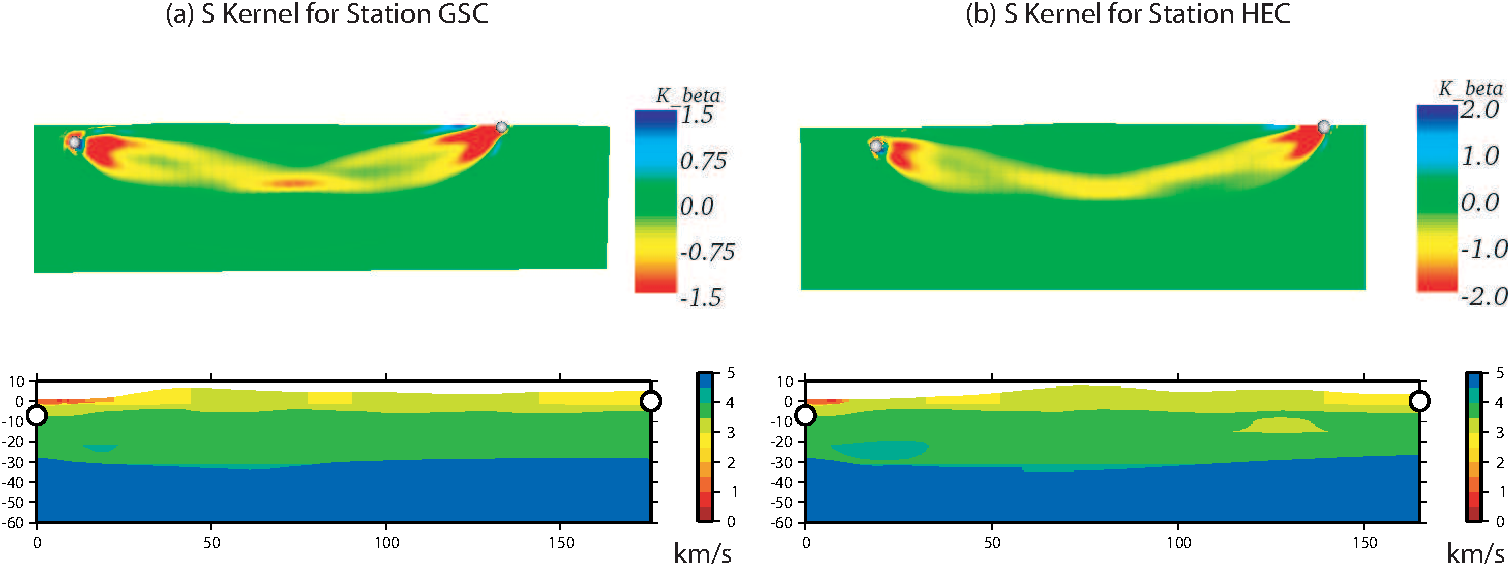
\includegraphics[scale=0.6]{figures/3D-S-Kernel.pdf}
\par\end{centering}

\caption{(a) Top Panel: Vertical source-receiver cross-section of the S-wave
finite-frequency sensitivity kernel $K_{\beta}$ for station GSC at
an epicentral distance of 176 km from the September 3, 2002, Yorba
Linda earthquake. Lower Panel: Vertical source-receiver cross-section
of the 3D S-wave speed model used for the spectral-element simulations
\citep{KoLiTrSuStSh04}. (b) The same as (a) but for station HEC at
an epicentral distance of 165 km \citep{LiTr06}.}


\label{figure:P-wave-speed-finite-frequency}
\end{figure}


